\documentclass[11pt,a4paper,landscape]{article}
\usepackage[margin=17mm,headheight=14pt,includeheadfoot]{geometry}
\usepackage[T1]{fontenc}
\usepackage{newtxtext,newtxmath,microtype,graphicx,caption,fancyhdr,xcolor}
\usepackage{hyperref}
\definecolor{ink}{HTML}{23384D}
\hypersetup{colorlinks=true,linkcolor=ink,urlcolor=ink,pdftitle={KSIVI variance investigation: scientific figures}}
\pagestyle{fancy}\fancyhf{}
\fancyhead[L]{\small\itshape KSIVI on the X-shaped target}
\fancyhead[R]{\small Scientific evidence}
\fancyfoot[C]{\thepage}\renewcommand{\headrulewidth}{0.3pt}
\captionsetup{font=small,labelfont=bf,labelsep=period}
\setlength{\parindent}{0pt}
\begin{document}
\begin{figure}[!ht]
\centering
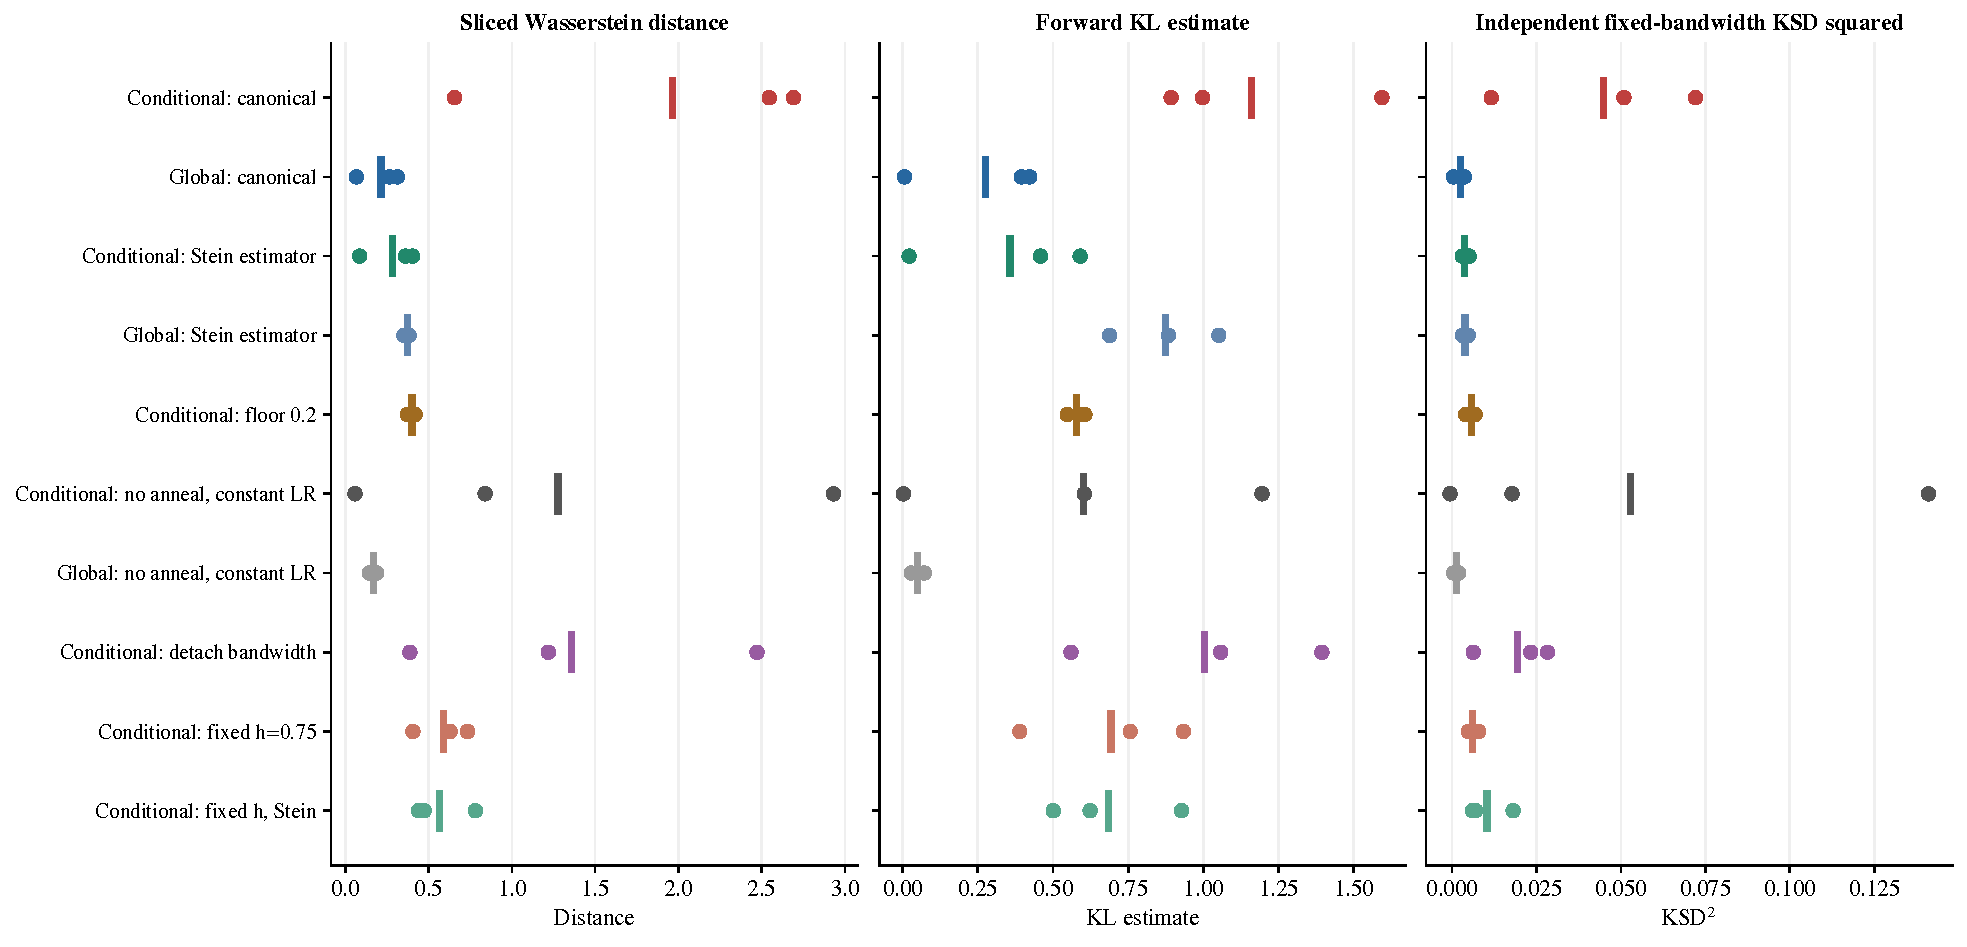
\includegraphics[width=\linewidth,height=.85\textheight,keepaspectratio]{figures/confirmation.pdf}
\caption{Matched comparisons after 50,000 updates. Dots are independently trained seeds 42--44; vertical strokes mark means. Initial mean weights, variance values, and training noise are paired. Forward KL uses the largest evaluated latent mixture; held-out KSD uses an independent fixed bandwidth of 0.75.}
\end{figure}

\clearpage
\begin{figure}[!ht]
\centering
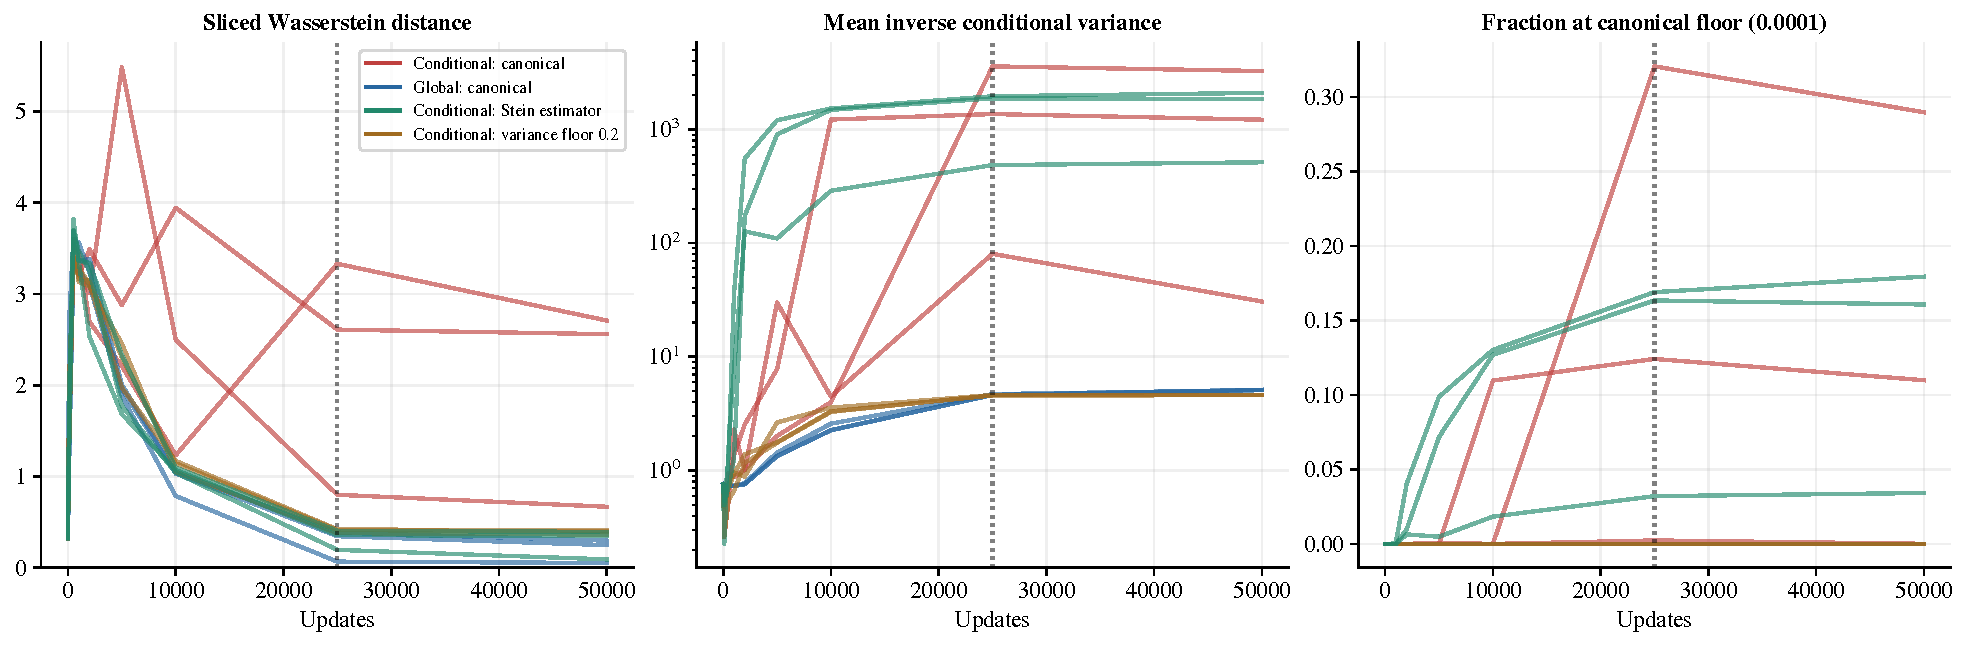
\includegraphics[width=\linewidth,height=.85\textheight,keepaspectratio]{figures/trajectories.pdf}
\caption{Accuracy and the small-variance tail across three trajectories per procedure. The dotted line marks completion of target annealing at update 25,000. Floor occupancy uses the common threshold 0.00010001; diagnostic draws preserve training RNG.}
\end{figure}

\clearpage
\begin{figure}[!ht]
\centering
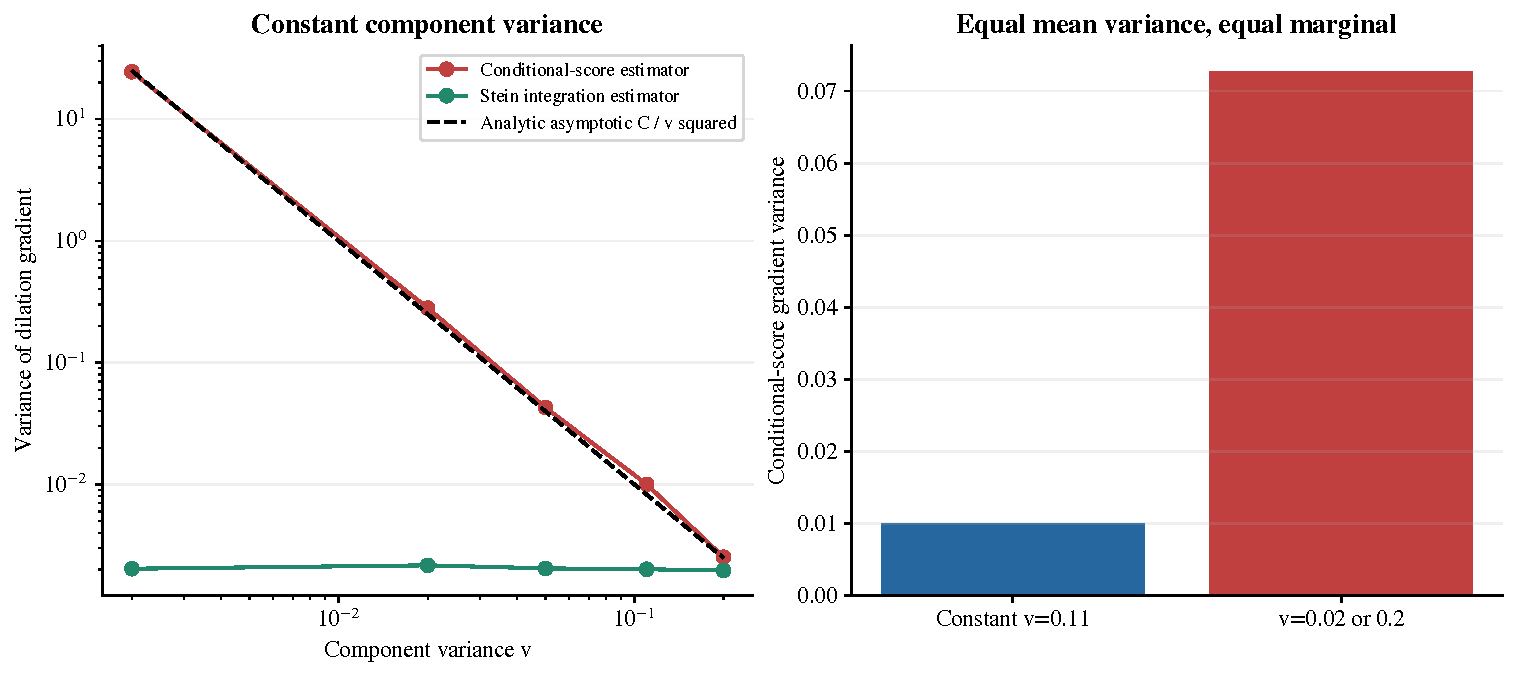
\includegraphics[width=\linewidth,height=.85\textheight,keepaspectratio]{figures/exact_marginal_noise.pdf}
\caption{Representation noise at exactly equal marginal distributions. Each measurement uses 256 independent repetitions and two batches of 128 at fixed bandwidth 0.75. The dashed curve is the analytic small-variance prediction, with no fitted coefficient. The right panel holds both the marginal and mean component variance 0.11 fixed.}
\end{figure}

\clearpage
\begin{figure}[!ht]
\centering
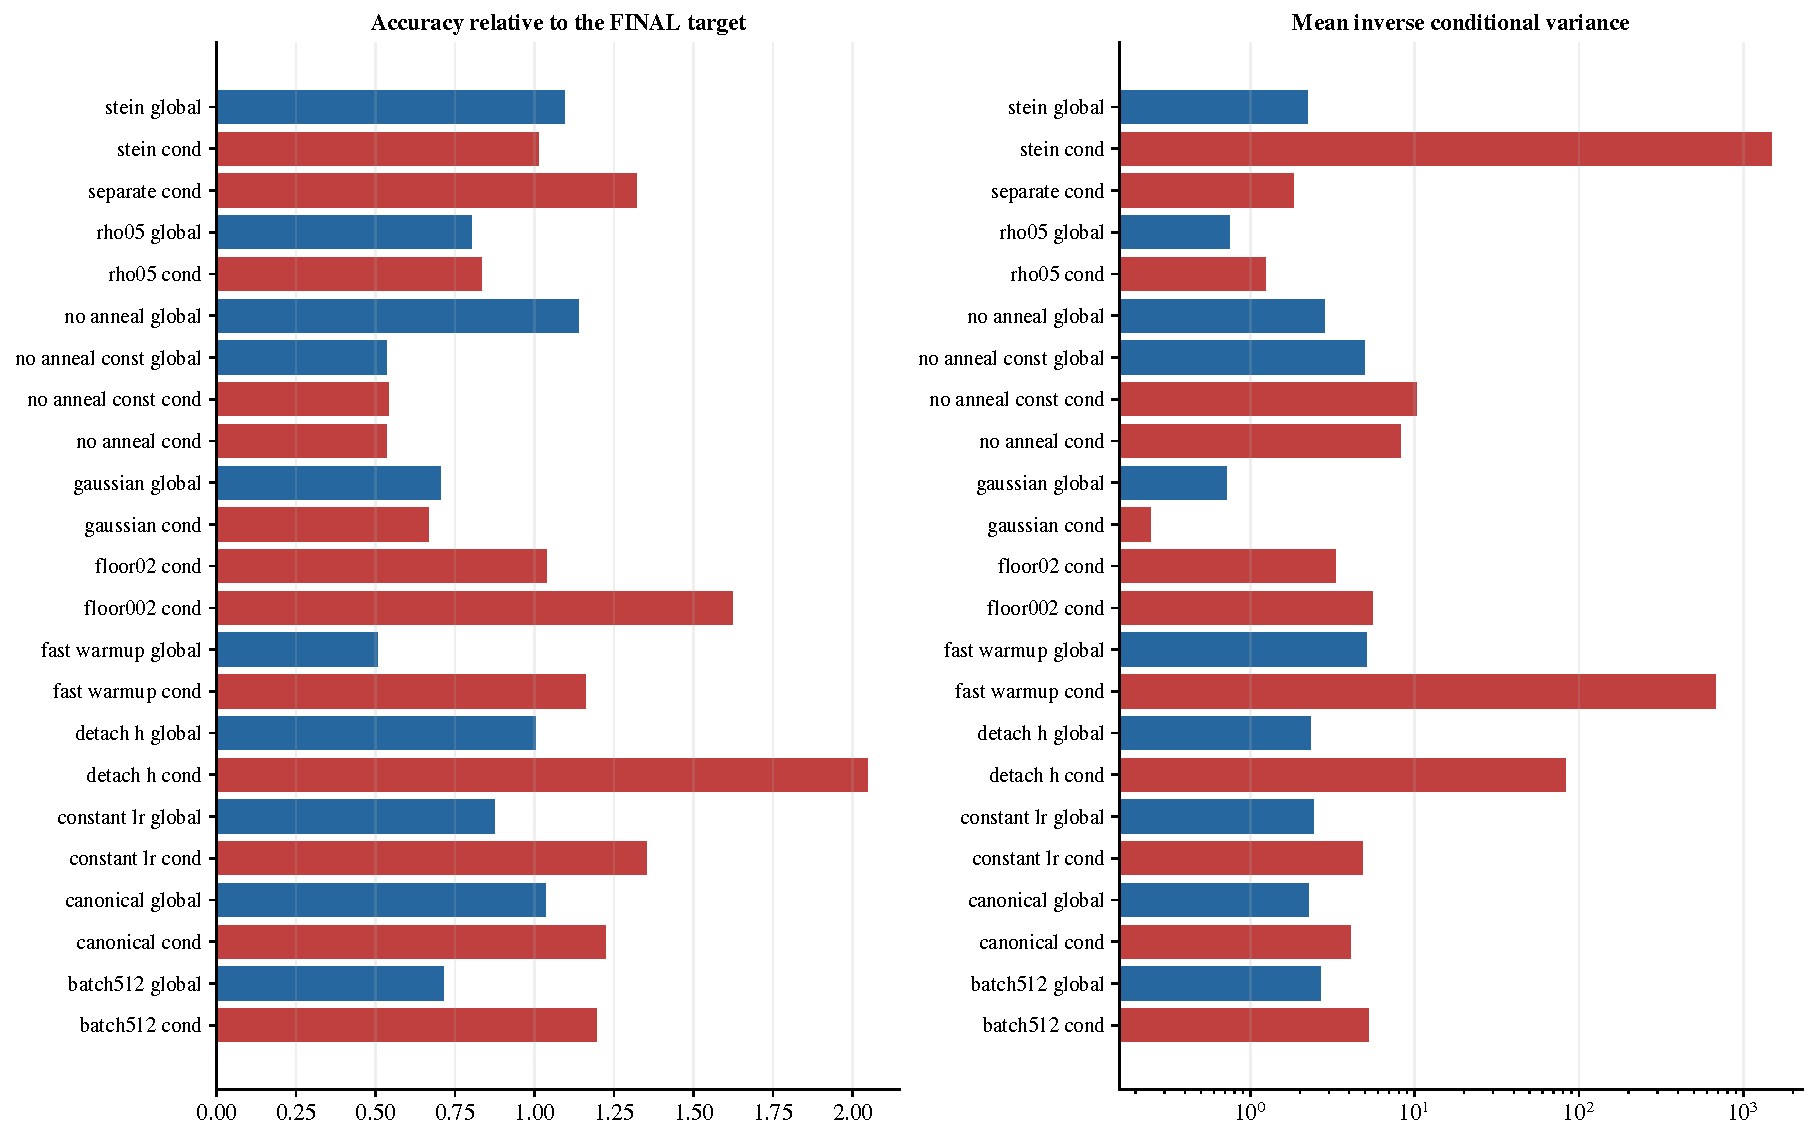
\includegraphics[width=\linewidth,height=.85\textheight,keepaspectratio]{figures/screening.pdf}
\caption{All 23 screening outcomes at 10,000 updates, seed 42. Blue denotes global variance; red denotes conditional variance. Annealed runs still have a score multiplier of 0.46 unless warmup is shortened. Distances are measured against the final target and do not establish final-target convergence.}
\end{figure}

\clearpage
\begin{figure}[!ht]
\centering
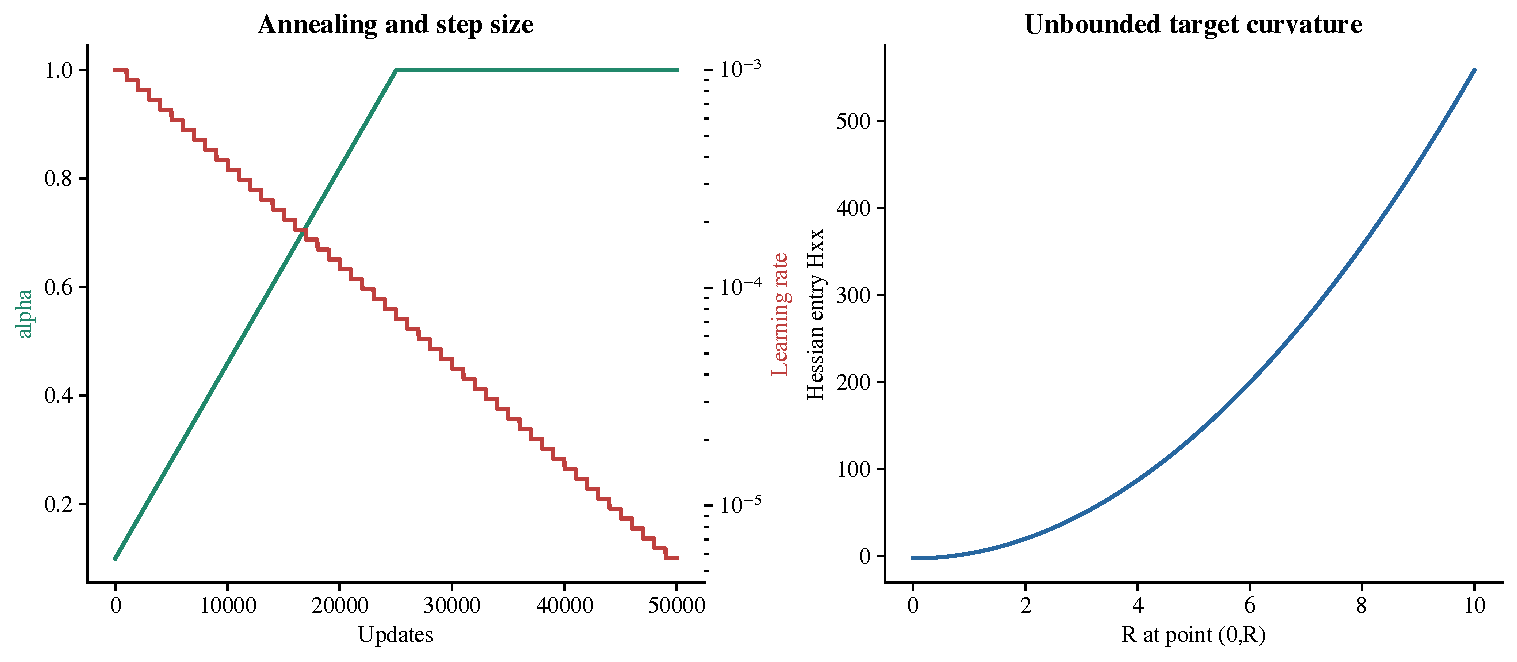
\includegraphics[width=\linewidth,height=.85\textheight,keepaspectratio]{figures/geometry_and_schedule.pdf}
\caption{Target path, learning-rate decay, and target curvature. The score multiplier reaches one after the learning rate has fallen to approximately 0.0000718. The diverging Hessian entry violates the global bounded-Hessian assumption for both variational families; this fact alone does not explain their ordering.}
\end{figure}

\clearpage
\begin{figure}[!ht]
\centering
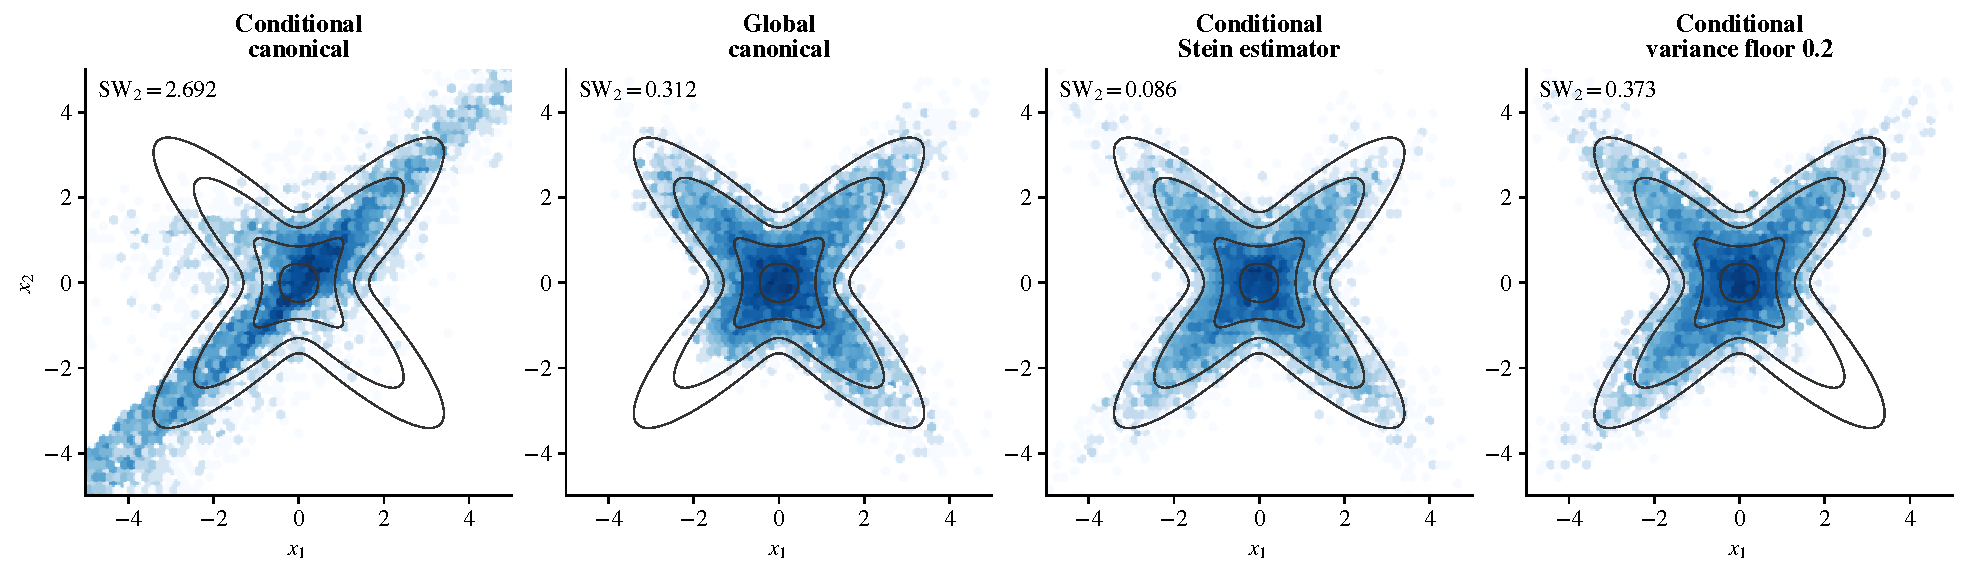
\includegraphics[width=\linewidth,height=.85\textheight,keepaspectratio]{figures/final_samples_s42.pdf}
\caption{Final samples, seed 42, after 50,000 updates. Black curves are exact target contours. All four procedures use matched initial mean functions and variance values. The common viewing window omits some tails, which remain included in all numerical metrics.}
\end{figure}

\clearpage
\begin{figure}[!ht]
\centering
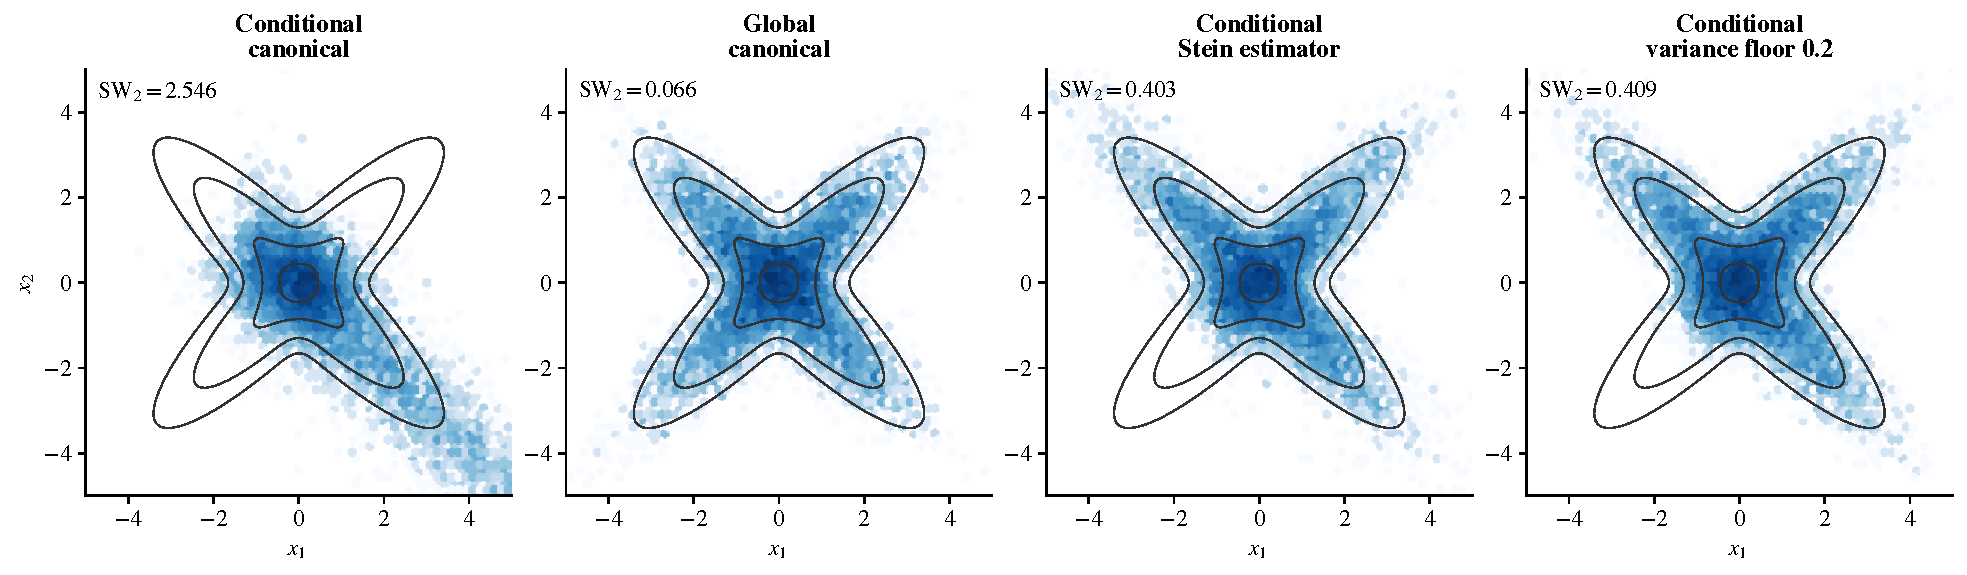
\includegraphics[width=\linewidth,height=.85\textheight,keepaspectratio]{figures/final_samples_s43.pdf}
\caption{Final samples, seed 43, after 50,000 updates. Black curves are exact target contours. All four procedures use matched initial mean functions and variance values. The common viewing window omits some tails, which remain included in all numerical metrics.}
\end{figure}

\clearpage
\begin{figure}[!ht]
\centering
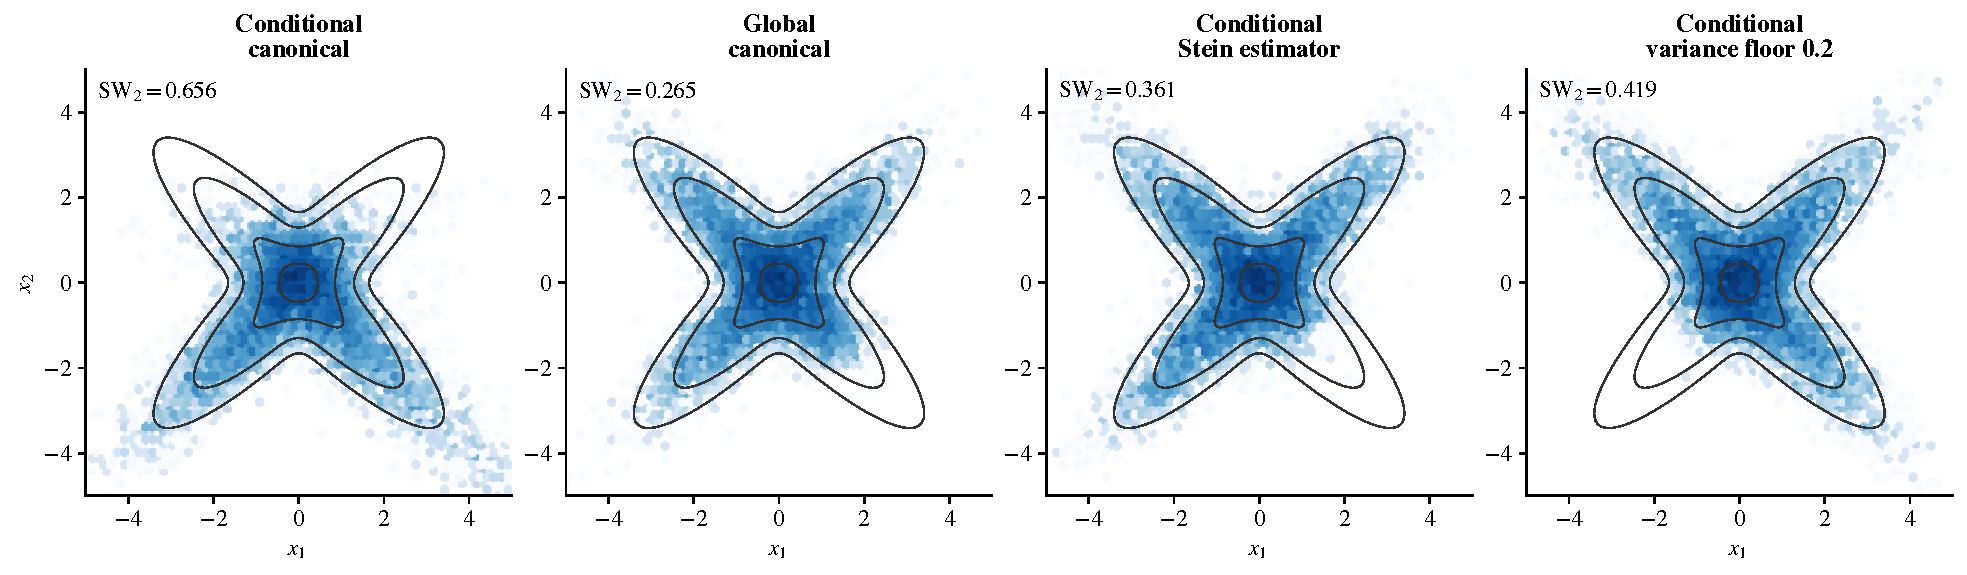
\includegraphics[width=\linewidth,height=.85\textheight,keepaspectratio]{figures/final_samples_s44.pdf}
\caption{Final samples, seed 44, after 50,000 updates. Black curves are exact target contours. All four procedures use matched initial mean functions and variance values. The common viewing window omits some tails, which remain included in all numerical metrics.}
\end{figure}
\end{document}
